%\documentclass[12pt, preprint,numberedappendix]{emulateapj}
%\documentclass[12pt, preprint]{aastex}
%\documentclass[dvips,12pt]{article}
\documentclass[apj]{emulateapj}

\newcommand\submitms{n}		% set to y to follow AAS ``ms'' names, etc.
\newcommand\bibinc{n}		% set to y if bib pasted in .tex, set to n to use bibtex


%\usepackage{pdfsync}
\usepackage{subeqnarray}
\usepackage{natbib}
\usepackage{color}
\usepackage[utf8]{inputenc}

\bibliographystyle{apj}

\newcommand{\ie}{i.e.\ }
\newcommand{\eg}{e.g.\ }
\newcommand{\p}{\partial}
\newcommand{\brak}[1]{\langle #1\rangle}


\newcommand{\gcc}{\;\mathrm{g\; cm^{-3}}}
\newcommand{\gsc}{\;\mathrm{g\; cm^{-2}}}
\newcommand{\cm}{\; {\rm cm}}
\newcommand{\mm}{\; {\rm mm}}
%\newcommand{\ps}{\; {\rm s^{-1}}}
\newcommand{\km}{\; {\rm km}}
\newcommand{\au}{\; \varpi_{\rm AU}}
\newcommand{\AU}{\; {\rm AU}}
\def\K{\; {\rm K}}

\newcommand{\vcs}[1]{\mbox{\boldmath{$\scriptstyle{#1}$}}}
\newcommand{\vc}[1]{\mbox{\boldmath{$#1$}}}
\newcommand{\nab}{\vc{\nabla}}
\DeclareMathSymbol{\varOmega}{\mathord}{letters}{"0A}
\DeclareMathSymbol{\varSigma}{\mathord}{letters}{"06}
\DeclareMathSymbol{\varPsi}{\mathord}{letters}{"09}

\newcommand{\Eq}[1]{Equation\,(\ref{#1})}
\newcommand{\Eqs}[2]{Equations (\ref{#1}) and~(\ref{#2})}
\newcommand{\Eqss}[2]{Equations (\ref{#1})--(\ref{#2})}
\newcommand{\App}[1]{Appendix~\ref{#1}}
\newcommand{\Sec}[1]{Sect.~\ref{#1}}
\newcommand{\Chap}[1]{Chapter~\ref{#1}}
\newcommand{\Fig}[1]{Fig.~\ref{#1}}
\newcommand{\Figs}[2]{Figs.~\ref{#1} and \ref{#2}}
\newcommand{\Figss}[2]{Figs.~\ref{#1}--\ref{#2}} 
\newcommand{\Tab}[1]{Table \ref{#1}}

\definecolor{gray}{gray}{0.5}
\newcommand{\emgr}[1]{\emph{ \color{gray} #1}}


%\newenvironment{packed_item}{
%\begin{itemize}
%  \setlength{\itemsep}{1pt}
%  \setlength{\parskip}{0pt}
%  \setlength{\parsep}{0pt}
%}{\end{itemize}}

\begin{document}

%\slugcomment{Draft Modified \today}


\title{The Role of Ice Compositions and Morphology for Snowlines and the C/N/O Ratios in Active Disks}

\author{Ana-Maria A. Piso\altaffilmark{1}, Karin I. \"Oberg\altaffilmark{1}, Jamila Pegues\altaffilmark{2}}
\altaffiltext{1}{Harvard-Smithsonian Center for Astrophysics, 60 Garden Street, Cambridge, MA 02138}
\altaffiltext{2}{Department of Astrophysical Sciences, Princeton University}


\begin{abstract}
The elemental compositions of planets define their chemistry, and could potentially be used as beacons for their formation location if the elemental gas and grain ratios of planet birth environments, i.e. protoplanetary disks, are well understood. In disks, the ratios of volatile elements, such as C/O and N/O, are regulated by the abundance of the main C, N, O carriers, the ice environment in which these carriers reside, and the presence of snowlines of major volatiles at different distances from the central star. We explore the effects of dynamical processes, molecular compositions and abundances, and the ice morphology of dust grains in disks on the snowline locations of the main C, O and N carriers, and their consequences for the C/N/O ratios in gas and dust throughout the disk. We find that radial drift and accretion alone can reduce the snowline radii of the main C, O and N carriers, i.e. H$_2$O, CO$_2$, CO and N$_2$, by 40-60\% compared to static disks. If CO and N$_2$ are water dominated instead of pure ices, their snowlines move inward by $\sim$$70$\%. Both of these effects substantially change the disk regions where gas phase C/O and N/O are enhanced over the stellar value, and taken together they may move the CO and N$_2$ snowlines by a factor of $\sim$7 inward. In the outer disk, the gaseous C/O and N/O are enhanced by factors of $\sim$$2$ and $\sim$$3$, respectively. Our estimates for the C/N/O ratios are only modestly affected by the presence of some C in the form of CH$_4$ and of some N in the form of NH$_3$.  

%We note that N/O enhancements in disk gas can be even more extreme than C/O in the outer disk due to the low volatility of N2 compared to all major C and O carriers. I will discuss these results together with the effects of additional dynamical processes, and outline a path toward a coupled drift-desorption-chemistry model that will provide robust quantitative results for volatile snowline locations and C/N/O abundance ratios as the disk evolves in time.
\end{abstract}

\section{Introduction}
\label{sec:intro}

%\begin {enumerate}
The chemical composition of protoplanetary disks is largely dictated by the freeze-out of volatile species, such as carbon, oxygen and nitrogen carriers. The snowline locations of volatile molecules are crucial in determining disk chemical abundances in gas and dust, as well as planet compositions.  

Carbon and oxygen bearing molecules, such as H$_2$O, CO$_2$ and CO, as well as the carbon-to-oxygen (C/O) ratio in protoplanetary disks and in giant planet atmospheres have been extensively studied from a theoretical standpoint (\citealt{oberg11}, \citealt{alidib14}, \citealt{madhu14}, \citealt{molliere15}), and snowlines of volatiles such as H$_2$O and CO have been detected (\citealt{zhang13}, \citealt{qi13}). However, disk chemistry is complex, and it involves many species besides carbon and oxygen carriers \citep{henning13}. In particular, several other volatiles have been detected in disks, such as nitrogen bearing species and hydrocarbons (e.g., \citealt{mandell12}), which adds further complexity to the disk composition.

 %However, both observations and chemical models (refs) have shown that other volatiles are abundant in disks, for example nitrogen bearing species and hydrocarbons, thus shaping the disk composition.

Moreover, snowline locations strongly depend on the grain morphology and the ice environment in which the grains reside. Laboratory experiments (\citealt{fayolle16}) have shown that volatiles such as CO and N$_2$ have significantly different binding energies depending on whether they are pure or water dominated ices. This implies that ices in different environments will sublimate at different radii, which will substantially change the disk regions where these volatiles are present in gaseous or solid form (see Sections \ref{sec:CH4} and \ref{sec:N}).  

 It follows that there are several important snowlines in disks, determined both by the disk composition and ice morphology. Figure \ref{fig:CNOstatic} shows an example of the H$_2$O, CO$_2$, CO, CH$_4$, NH$_3$ and N$_2$ snowlines in a static disk, with CO and N$_2$ as pure and water dominated ices, in the top and bottom panel, respectively. The ordinate displays the total carbon, oxygen and nitrogen abundance in solids as a function of the hydrogen abundance. We note that we display this Figure here for qualitative purposes; the quantitative choices that we make for volatile abundances are discussed in Sections \ref{sec:CH4} and \ref{sec:N}. As expected, the total grain abundance increases with semimajor axis, as more and more species sublimate. More importantly, the CO and N$_2$ snowlines move several tens of AU inward if the ices are water dominated rather than pure. This changes the chemical abundances both in gas and dust throughout the disk, directly affecting the compositions of nascent giant planets forming in situ. 
 
% Disk dynamical processes such as radial drift of solids and viscous gas accretion onto the central store also change the position of the snowlines, as demonstrated by \citet{piso15b} (hereafter Paper I), which introduces another element of uncertainty in the snowline locations. 

In order to explain this added chemical and physical complexity, a more thorough theoretical framework is needed. In this work, we expand the coupled drift-desorption model developed in \citet{piso15b} (hereafter Paper I) by considering additional volatile molecules and abundances, and ice morphology, in addition to disk dynamical processes. 

This paper is organized as follows. In Section \ref{sec:review}, we review the drift-desorption model developed in Paper I. We discuss the effect of different abundances of the main carbon and oxygen carriers, grain morphology and dynamical processes on the snowline locations of carbon and oxygen bearing species and the C/O ratio in Section \ref{sec:CH4}. In Section \ref{sec:N}, we perform the same analysis for the main nitrogen carriers and the nitrogen-to-oxygen (N/O) ratio. We summarize our findings in Section \ref{sec:summary}.  

%\end {enumerate}

%\emgr{Background info. Importance of volatiles in disks and planetary atmospheres, detections of snowlines in disks, C/O ratios etc. State again the importance of radial drift and gas accretion on the snowline locations, and that a systematic study of the combination of these two particular effects across the disk has not been done before. Then transition to the fact that we provide such a systematic study in Paper I and in this paper. Here, we expand the model of Paper I by making three additions: (1) we add N and CH4 in the static chemistry model, and explore how different abundances of CH4 and of the N main carriers (N2 and NH3) affect the C/O  and N/O ratios, (2) we quantify the effect of radial drift and gas accretion on the N2, CH4 and NH3 snowline locations, and (3) we explore how different binding energies of CO and N2 affect their snowline locations.}

\begin{figure*}[t!]
\centering
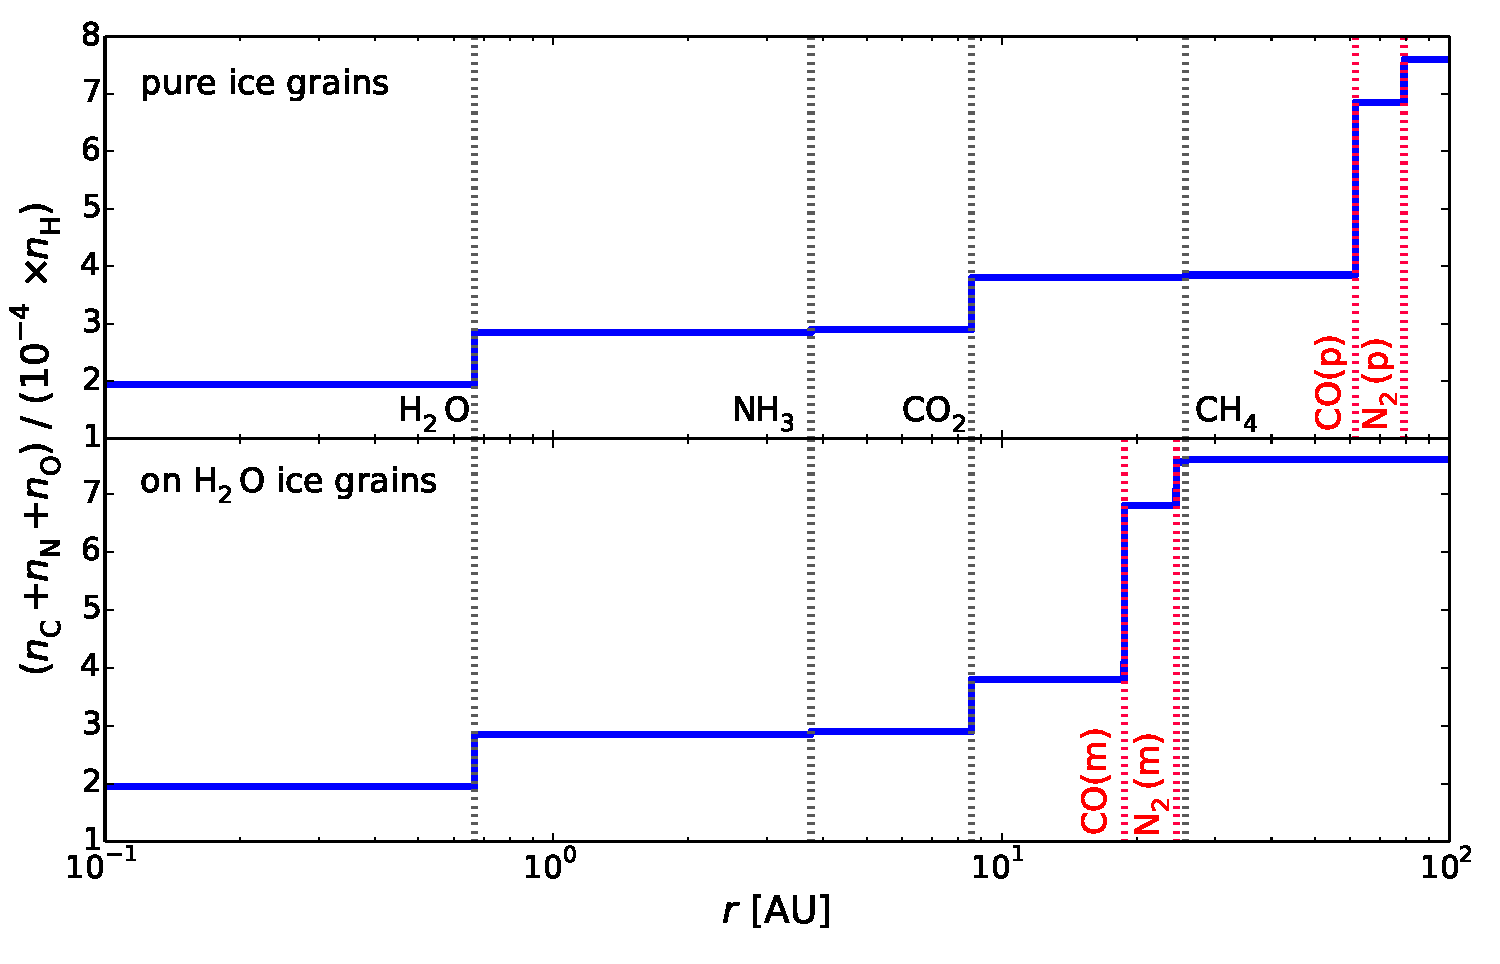
\includegraphics[width=\textwidth]{CNO_and_snowlines_2.pdf}
%\vspace{-0.5in}
\caption{The total carbon, nitrogen and oxygen abundance as a function of semimajor axis in a static disk, for CO and N$_2$ as pure ices (top panel) and water dominated ices (bottom panel). Relevant volatile snowlines are marked by the vertical dashed lines. The grain abundances are calculated as a function of the observed median CH$_4$ and NH$_3$ abundances in protostellar cores (see Sections \ref{sec:CH4} and \ref{sec:N}). The total grain abundance increases with semimajor axis as more and more species freeze out.} 
\label{fig:CNOstatic}
\end{figure*}

\section{Coupled Drift-Desorption Model Review}
\label{sec:review}

We begin with a brief review of Paper I's model for the effect of radial drift and viscous gas accretion on volatile snowline locations. We review our disk model in Section \ref{sec:disktime}, and summarize our numerical method and results in Section \ref{sec:driftdes}.

\subsection{Disk Model}
\label{sec:disktime}

We first assume a static disk, which is only irradiated by the central star and does not experience redistribution of solids or radial movement of the nebular gas. To quantify the effects of radial drift and gas accretion, we use a viscous disk with a spatially and temporally constant mass flux, $\dot{M}$. The viscous disk takes into account radial drift, gas accretion onto the central star, as well as accretion heating. We prefer this disk model to an irradiated or evolving disk (see Paper I) because it includes all the dynamical and thermal processes we are interested in for the scope of this paper, and therefore it is the most realistic one.  

Following \citet{chiang10}, the temperature profile for a static disk is
\begin{equation}
\label{eq:diskT}
T = 120\, (r/\text{AU})^{-3/7} \,\,\text{K},
\end{equation}
%We model the static disk as a minimum mass solar nebula (MMSN), using a prescription for the gas surface density, $\Sigma$, and disk midplane temperature, $T$, similar to that of \citet{chiang10}:
%\begin{subeqnarray}
%\label{eq:disk}
%\Sigma&=&2000\, (r/\text{AU})^{-1}\,\, \text{g cm}^{-2} \slabel{eq:disksigma}\\
%T &=& 120\, (r/\text{AU})^{-3/7} \,\,\text{K}, \slabel{eq:diskT}
%\end{subeqnarray}
where $r$ is the semimajor axis. We use the \citet{shakura73}  steady-state disk solution to model the viscous disk. From Paper I, the viscous disk temperature profile is computed as % Solving the Equation set of Appendix A in Paper I yields an expression for the temperature profile in a steady-state disk:
\begin{equation}
\label{eq:activeT}
T^4 =\Big[\frac{1}{4 r} \Big(\frac{3 G \kappa_0\dot{M}^2 M_* \mu m_{\rm p} \Omega_{\rm k}}{\pi^2 \alpha k_{\rm B} \sigma}\Big)^{1/3}\Big]^4 + T_{\rm irr}^4,
\end{equation}
where $T_{\rm irr}=T$ from Equation (\ref{eq:diskT}). Here $G$ is the gravitational constant, $\kappa_0=2 \times 10^{-6}$ is a dimensionless opacity coefficient, $M_*=M_{\odot}$ is the mass of the central star, $\mu=2.35$ is the mean molecular weight of the nebular gas, $m_{\rm p}$ is the proton mass, $\Omega_{\rm k}=\sqrt{G M_{\odot}/r^3}$ is the Keplerian angular velocity, $\alpha=0.01$ is a dimensionless coefficient (see below for details), $k_{\rm B}$ is the Boltzmann constant, and $\sigma$ is the Stefan-Boltzmann constant. 

%The final midplane temperature profile is computed as 
%\begin{equation}
%\label{eq:activeT}
%T^4 = T_{\rm act}^4 + T_{\rm irr}^4,
%\end{equation}
%where $T_{\rm irr}=T$ from Equation (\ref{eq:diskT}). We use this expression because in addition to accretion heating, stellar irradiation also contributes to the disk thermal structure. 

The steady-state disk has an $\alpha$-viscosity prescription, where the kinematic viscosity is $\nu=\alpha c H$. Here $c \equiv \sqrt{k_{\rm B} T /(\mu m_{\rm p})}$ is the isothermal sound speed (with $T$ from Equation \ref{eq:activeT}), and $H \equiv c/\Omega_{\rm k}$ is the disk scale height. We can then determine the gas surface density for a viscous disk as (\citealt{shakura73}; see also Paper I for a more detailed explanation of these calculations):
\begin{equation}
\label{eq:Sigmaact}
\Sigma=\frac{\dot{M}}{3 \pi \nu}.
\end{equation}
We choose $\dot{M}=10^{-8} M_{\odot}$ yr$^{-1}$, consistent with mass flux observations in disks (e.g., \citealt{andrews10}). As acknowledged in Paper I, the mass flux rate $\dot{M}$ and stellar luminosity $L_*$ will vary throughout the disk lifetime (\citealt{kennedy06}, \citealt{chambers09}), in contrast with our simplified model which assumes that both quantities are constant. This effect will be most pronounced in the inner disk ($\lesssim$ few AU), where accretion heating dominates. We thus acknowledge that the location of the H$_2$O snowline may be determined by the decline in $\dot{M}$ or $L_*$ with time, rather than radial drift (see Paper I, Section 2.1 for a more detailed explanation). 

%In what follows, we summarize the relevant timescales that affect volatile snowline locations. 
%
%\textit{Desorption timescale.} Following \citet{hollenbach09} and Paper I, the timescale to desorb a single layer of molecules of a volatile $x$ can be approximated as
%\begin{equation}
%\label{eq:tdes}
%t_{\rm des}=\frac{\rho_{\rm s}}{3 \mu_x m_{\rm p}} \frac{s}{N_x R_{\rm des, x}},
%\end{equation} 
%where $\rho_{\rm s}=2$ g cm$^{-3}$ is the density of an icy particle, $s$ is the particle size, $\mu_x$ is the mean molecular weight of volatile $x$, and $N_x \approx 10^{15}$ sites cm $^{-2}$ is the number of adsorption sites of molecule $x$ per cm$^{-2}$. The desorption rate $R_{\rm des, x}$ (per molecule) is \citep{hollenbach09}
%\begin{equation}
%\label{eq:Rdes}
%R_{\rm{des}, x} = \nu_x \exp{(-E_x/T_{\rm grain})},
%\end{equation}
%where $E_x$ is the adsorption binding energy in units of Kelvin, $T_{\rm grain}=T$ is the grain temperature (assumed to be the same as the disk temperature, see Paper I), and $\nu_x=1.6 \times 10^{11} \sqrt{(E_x/\mu_x)}$ s$^{-1}$ is the molecule's vibrational frequency in the surface potential well. We discuss our choices for $E_x$ for the different volatile species in Sections \ref{sec:CH4} and \ref{sec:N}.

\subsection{Desorption-Drift Equations and Results}
\label{sec:driftdes}

For a range of initial icy grain sizes composed of a single volatile, we showed in Paper I that the timescale on which these particles desorb is comparable to their radial drift time, as well as to the accretion timescale of the nebular gas onto the central star. We thus have to take into account both drift and gas accretion when we calculate the disk location at which a particle desorbs, since that location may be different from the snowline position in a static disk for a given volatile (see Figure \ref{fig:CNOstatic} and \citealt{oberg11}). We determine a particle's final location in the disk by solving the following coupled differential equations:
\begin{subeqnarray}
\label{eq:ddt}
\frac{ds}{dt} &= & - \frac{3 \mu_x m_{\rm p}}{\rho_{\rm s}} N_x R_{\rm des, x}  \slabel{eq:dsdt} \\
\frac{dr}{dt} &=& \dot{r} \slabel{eq:drdt},
\end{subeqnarray}
where $s$ is the particle size, $t$ is time, $\mu_x$ is the mean molecular weight of volatile $x$, $\rho_{\rm s}=2$ g cm $^{-3}$ is the density of an icy particle, $N_x \approx 10^{15}$ sites cm $^{-2}$ is the number of adsorption sites of molecule $x$ per cm$^{-2}$, $R_{\rm des, x}$ is the desorption rate of species $x$, and $\dot{r}$ is the particle's radial drift velocity. We calculate $R_{\rm, des}$ and $\dot{r}$ as follows.

The desorption rate $R_{\rm des, x}$ (per molecule) is \citep{hollenbach09}
\begin{equation}
\label{eq:Rdes}
R_{\rm{des}, x} = \nu_x \exp{(-E_x/T_{\rm grain})},
\end{equation}
where $E_x$ is the adsorption binding energy in units of Kelvin, $T_{\rm grain}=T$ is the grain temperature (assumed to be the same as the disk temperature, see Paper I), and $\nu_x=1.6 \times 10^{11} \sqrt{(E_x/\mu_x)}$ s$^{-1}$ is the molecule's vibrational frequency in the surface potential well. We discuss our choices for $E_x$ for the different volatile species in Sections \ref{sec:CH4} and \ref{sec:N}.

Following \citet{chiang10} and \citet{birnstiel12}, a particle's radial drift velocity can be approximated as 
\begin{equation}
\label{eq:rdotact}
\dot{r} \approx -2 \eta \Omega_{\rm k} r \Big(\frac{\tau_{\rm s}}{1+\tau_{\rm s}^2}\Big) + \frac{\dot{r}_{\rm gas}}{1+\tau_{\rm s}^2},
\end{equation}
where the first term is the drift velocity in a non-accreting disk and the second term accounts for the radial movement of the gas. Here $\eta \approx c^2/(2 v_{\rm k}^2)$, where $v_{\rm k}$ is the Keplerian velocity, and $\tau_{\rm s} \equiv \Omega_{\rm k} t_{\rm s}$ is the dimensionless stopping time:
\begin{equation}
\label{eq:ts}
t_{\rm s}= \left\{
\begin{array}{l l}
\rho_{\rm s} s / (\rho c), & \quad s < 9 \lambda/4 \,\,\,\ \text{Epstein drag} \\
4 \rho_{\rm s} s^2 / (9 \rho c \lambda), & \quad s < 9 \lambda/4, \,\text{Re} \lesssim 1 \,\,\,\ \text{Stokes drag,}
\end{array} 
\right.
\end{equation}
where $\rho$ is the disk mid-plane density, $\lambda$ is the mean free path and Re is the Reynolds number.  The gas accretion velocity $\dot{r}_{\rm gas}$ is determined from $\dot{M}=-2 \pi r \dot{r}_{\rm gas} \Sigma$, for a fixed $\dot{M}$ and with $\Sigma$ given by Equation (\ref{eq:Sigmaact}). 

For a particle of initial size $s_0$, we solve the Equation set (\ref{eq:ddt}) with the initial conditions $s(t_0)=s_0$ and $r(t_0)=r_0$, where $t_0$ is the time at which we start the integration and $r_0$ is the particle's initial location. We stop our simulation after $t_{\rm d}=3$ Myr, the disk lifetime, since this is roughly the timescale on which planets form, and determine the desorption timescale $t_{\rm des}$ from $s(t_{\rm des})=0$, and thus a particle's desorption distance $r_{\rm des}=r(t_{\rm des})$. Our results are insensitive to our choice of $t_0$ as long as $t_0 \ll t_{\rm d}$. We note that a particle's size is initially fixed and only changes due to desorption. We thus do not take into account processes such as grain coagulation or fragmentation, which nonetheless occur in disks (e.g., \citealt{birnstiel12}, \citealt{perez12}). We discuss the effect of these processes on snowline locations in Paper I.

As we show in Paper I, a particle of initial size $s_0$ can experience three outcomes after $t_{\rm d}=3$ Myr: (1) it can remain at its initial location, (2) it can drift towards the host star, then stop without evaporating significantly, and (3) it can completely desorb on a timescale shorter than 3 Myr. Particles in scenarios (1) and (2) are thus not affected by radial drift or gas accretion, and the snowline locations are those for a static disk. In contrast, the grains in case (3) desorb \textit{instantaneously} and \textit{at a fixed particle-size dependent location} in the disk, regardless of their initial position. The snowline locations for these particles will thus be fixed for a given initial particle size and disk model. We have found that grains with sizes $\sim0.001$ cm $\lesssim s \lesssim$ 7 m satisfy this condition for our fiducial disk. 

%\emgr{Review disk models, desorption model, relevant timescales. State that we use a steady-state disk for the coupled drift-desorption evolution, since it is the most realistic, therefore only summarize the static and steady-state (viscous) disk. Summarize the findings of Paper I, i.e. particles of certain sizes desorb instantaneously and at a fixed particle size dependent location.}

\section{The Effect of CO Ice Morphology and CH$_4$ on the C/O Ratio}
\label{sec:CH4}

\subsection{Role of CH$_4$}

Both in Solar system comets and in protoplanetary disks, carbon and oxygen are primarily contained in H$_2$O, CO$_2$ and CO (e.g., \citealt{rodgers02}, \citealt{lodders03}, \citealt{pontoppidan06}). However, some fraction of the carbon abundance may also be carried by CH$_4$ (e.g., \citealt{mumma96}), which may change the C/O ratio in gas and in dust throughout the disk. To quantify the magnitude of this effect, we use measured CH$_4$ abundances in protostellar cores from the \textit{Spitzer} c2d Legacy ice survey \citep{evans03}. We explore the parameter space of possible CH$_4$ abundances by assuming three different scenarios: (1) no CH$_4$, (2) the median CH$_4$ observed abundance (hereafter CH$_4$-mid), and (3) the maximum CH$_4$ observed abundance (hereafter CH$_4$-max). Thus $n_{\rm CH_4-mid}=0.0555 \times n_{\rm H_2O}$ \citep{oberg11a} and $n_{\rm CH_4-max}=0.13 \times n_{\rm H_2O}$ \citep{oberg08}, where $n_{\rm H_2O}$ is the total H$_2$O abundance. Similarly to Paper I, we use the H$_2$O, CO$_2$ and CO abundances of \citet{oberg11}. Since the abundance of carbon grains is uncertain, we assume that all the carbon that is not in the form of CH$_4$ is found in carbon grains, so that we reproduce the Solar C/O ratio (gas+dust) of 0.54.  

We determine the location of the H$_2$O, CO$_2$, CO and CH$_4$ snowlines in our static disk by balancing desorption with readsorption, following \citet{hollenbach09}. The binding energies of H$_2$O, CO$_2$, CO and CH$_4$ as pure ices are 5800 K, 2000 K, 834 K and 1300 K, respectively (\citealt{fraser01}, \citealt{collings04}, \citealt{fayolle16}, \citealt{garrod06}).

\begin{figure}[h!]
\centering
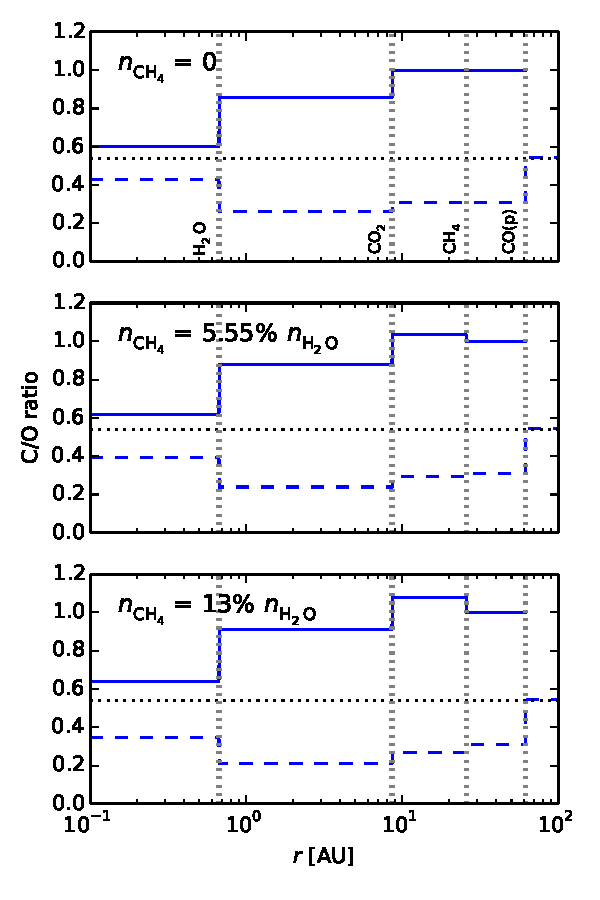
\includegraphics[width=0.5\textwidth]{C_O_ratio_CH4.pdf}
%\vspace{-0.5in}
\caption{The C/O ratio in gas (solid lines) and dust (dashed lines) as a function of semimajor axis in a static disk, assuming no carbon is present in the form of CH$_4$ (top panel), the median observed CH$_4$ abundance is assumed (middle panel), and the maximum observed CH$_4$ abundance is assumed (bottom panel). The C/O estimates are performed assuming that the CO ices are in pure form. The vertical dashed lines mark the snowline locations of the main C and O carriers. The horizontal dashed lines represent the stellar C/O value. The presence of methane only modestly increases the C/O ratio in gas between the CO$_2$ and CH$_4$ snowlines.} 
\label{fig:COstatic}
\end{figure}

Figure \ref{fig:COstatic} shows the C/O ratio in gas and dust as a function of semimajor axis in a static disk, for different CH$_4$ abundances as outlined above. As in \citet{oberg11} and Paper I, a gaseous C/O ratio of unity can be achieved beyond the CO$_2$ snowline, where oxygen gas is significantly depleted (top panel). The gas-phase C/O ratio may be further enhanced between the CO$_2$ and CH$_4$ snowlines due to the presence of additional carbon gas from CH$_4$. In this region, the C/O ratio increases by 3\% for CH$_4$-mid and by 8\% for  CH$_4$-max, as displayed in the middle and bottom panel of Figure \ref{fig:COstatic}. Based on current observations of CH$_4$ abundances, its presence in the disk only modestly affects the C/O ratio. Given the larger uncertainties in overall volatile abundances, we can neglect CH$_4$ when estimating the C/O ratio in static disks. %\footnote{This may not be the case, however, in a viscous disk, as we show below.}.  

\subsection{CO Ice Environment and Disk Dynamics}

As noted in Section \ref{sec:intro}, the CO binding energy varies significantly depending on the environment in which the icy grains reside. If CO ice is in a water dominated environment, its binding energy will be larger than in the pure ice case (834 K) due to the higher H$_2$O binding energy. \citet{fayolle16} find a CO binding energy of 1388 K in the water dominated ice scenario. We use the model of Section \ref{sec:review} to estimate the movement of the CO snowline for different grain morphologies in a viscous disk.

Figure \ref{fig:CO_ratio} shows the H$_2$O, CO$_2$ and CO snowline locations for particles with initial sizes $\sim0.06$ cm $\lesssim s \lesssim$ 7 m as well as estimates for the C/O ratio in gas and dust in a viscous disk, with the CO snowline calculated under different grain morphologies as noted above. The true snowline for particles that desorb outside the static snowline is the static snowline itself, hence desorbing particles with $s<0.06$ cm do not form true snowlines. As calculated in Paper I, drift and gas accretion may move the snowlines inwards by up to 40-60\% compared to a static disk, and specifically by up to $\sim50$ \% in the case of the CO snowline. This result is preserved for the updated CO binding energies, both for pure and water dominated ices. However, a water dominated environment moves the CO snowline inwards significantly: for our fiducial disk model, $r_{\rm CO, water} \approx 8.7$ AU. Thus if CO is water dominated instead of pure ice, the CO snowline may move inward by up to 70\%. By taking into account both disk dynamics and of CO in a water dominated environment, we find that the CO snowline may move inward by a factor of $\sim$$7$ compared to a static disk with CO as pure ice.  This large inward movement of the CO snowline implies that C/O ratios of order unity may be reached much closer to the host star if CO is a water dominated ice, and the CO snowline may be inside 10 AU for certain disk parameters.  

%\emgr{Discuss observed abundances for CH4 and the choices that we make (no CH4, median value, maximum value). State that desorption energies for H2O, CO2 and CH4 are well constrained experimentally, and that the CO2 and CH4 binding energies are only weakly dependent on whether it's pure CO2/CH4 or combined with H2O, but that is not the case for CO (and N2 as we will show in the next section). Present new binding energies for CO as pure ice and mixed with water. Show Figure 1 and discuss how different CH4 abundances and binding energies affect snowline locations and C/O ratio: CO-H2O mixture (though I think it's rather CO layered on top of H2O) moves the CO snowline inward by $\sim$40 AU (will calculate percentages too); the maximum reasonable abundance of CH4 changes the C/O ratio by less than 10\%. Show Figure 2 and quantify the effect of drift and accretion on the CH4 snowline compared to a static disk. While CH4 has only a modest effect on the C/O ratio in a static disk, this effect may be larger in a viscous disk, as the C gas abundances inside the CH4 snowline may be enhanced due to the differential motion of the desorbed ices and overall nebular gas (refer to Paper I). In this study, however, we neglect these effects and therefore do not include CH4 in estimating the C/O ratio (as an aside, the figures that include CH4 in the C/O ratio with drift and desorption are quite messy due to snowlines overlapping). Show Figure 3 and estimate the difference between CO-H2O and CO pure ice snowlines in the case of drift and accretion, as well as the comparisons for the static disk for the CO snowline.}


\begin{figure}[h!]
\centering
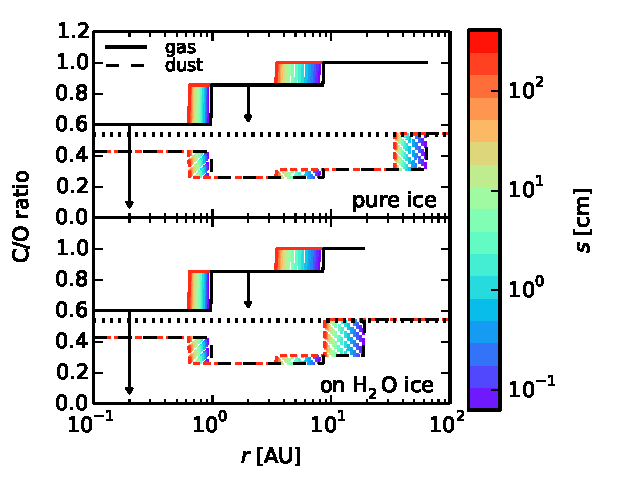
\includegraphics[width=0.5\textwidth]{C_O_water_ice.pdf}
%\vspace{-0.5in}
\caption{C/O ratio estimates in gas (solid lines) and dust (dashed lines) as function of semimajor axis in a viscous disk, for CO residing in a water ice environment (top panel) or as pure CO ice (bottom panel). The H$_2$O, CO$_2$ and CO snowlines are shown for particles with initial sizes $\sim0.001$ cm $\lesssim s \lesssim$ 7 m as indicated by the color bar. The C/O ratio in a static disk (black lines) is shown for comparison. The arrows show that the C/O ratio in gas will decrease inside the H$_2$O and CO$_2$
snowlines in the viscous disk, as the relative fluxes of the desorbed icy
particles and the overall nebular gas will cause an excess of oxygen gas inside these snowlines (see Paper I for details). Radial drift and gas accretion move the snowlines inward by 40-60\%. The presence of CO in a water ice environment rather than as pure ice moves the CO snowline significantly inward by $\sim$70\%.} 
\label{fig:CO_ratio}
\end{figure}

\section{The Effect of N$_2$ Ice Morphology on the N/O Ratio}
\label{sec:N}

\subsection{Nitrogen Carriers and the Role of NH$_3$}

In addition to carbon and oxygen, nitrogen is another abundant volatile in the Solar system and in disks. Chemical models of the protostellar nebula (e.g., \citealt{owen01}) and of protoplanetary disks (e.g., \citealt{rodgers02}) suggest that N$_2$ was the dominant form of nitrogen, and that giant planets have accreted their nitrogen content primarily as N$_2$ \citep{mousis14}. Observations of Solar system bodies such as Titan and Pluto show that N$_2$ is prevalent in their atmospheres (\citealt{cruikshank93}, \citealt{owen93}).  Moreover, the Rosetta spacecraft has recently made the first direct measurement of the N$_2$ abundance in comet 67P/Churyumov-Gerasimenko \citep{rubin15}. In addition to N$_2$, a fraction of the nitrogen abundances may be also carried by NH$_3$ (\citealt{bottinelli10}, \citealt{mumma11}). 

Because of the high volatility of N$_2$, the gas phase nitrogen-to-oxygen (N/O) ratio in the outer disk
may be even more enhanced than the C/O ratio compared to its average value in the disk. Giant planets that form at wide separations should thus have an excess of nitrogen in their atmospheres, which could be used to trace their formation origin.  In this study, we quantify this effect in protoplanetary disks. We assume that the main nitrogen-bearing species are N$_2$ and NH$_3$, since other volatiles that contain nitrogen have significantly lower abundances in comparison (e.g., \citealt{mumma11}). We use the measured total nitrogen abundance in the Solar system, $n_{\rm N}=8 \times 10^{-5} n_{\rm H}$ \citep{lodders03}, where $n_{\rm H}$ is the hydrogen abundance in the disk midplane. Similarly to the case of CH$_4$ (see Section \ref{sec:CH4}), we explore the parameter space of possible NH$_3$ abundances using data from the Spitzer c2d Legacy ice survey, as follows: (1) no NH$_3$, (2) the median NH$_3$ observed abundance $n_{\rm NH_3-mid}=0.055 \times n_{\rm H_2O}$ \citep{oberg11a}, and (3) the maximum observed NH$_3$ abundance $n_{\rm NH_3-max}=0.1537 \times n_{\rm H_2O}$ \citep{bottinelli10}. In each case, the N$_2$ abundance then simply follows as $n_{\rm N_2}=(n_{\rm N}-n_{\rm NH_3})/2$. We determine the locations of the N$_2$ and NH$_3$ snowlines by balancing desorption with readsorption \citep{hollenbach09}, with N$_2$ and NH$_3$ pure ice binding energies of  767 K and  2965 K, respectively (\citealt{fayolle16}, \citealt{martin14}). 

\begin{figure}[h!]
\centering
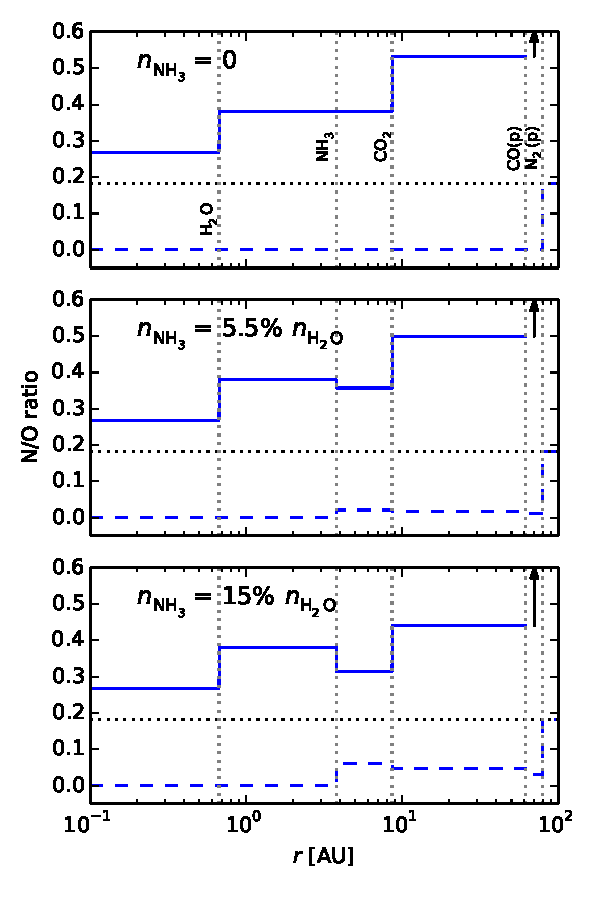
\includegraphics[width=0.5\textwidth]{N_O_ratio.pdf}
%\vspace{-0.5in}
\caption{The N/O ratio in gas (solid lines) and dust (dashed lines) as a function of semimajor axis in a static disk, assuming no nitrogen is present in the form of NH$_3$ (top panel), the median observed NH$_3$ abundance is assumed (middle panel), and the maximum observed NH$_3$ abundance is assumed (bottom panel). The N/O estimates are performed assuming that the CO and N$_2$ ices are in pure form. The vertical dashed lines mark the snowline locations of the main C,O and N carriers. The horizontal dashed lines represent the average N/O value in the disk. The gas-phase N/O ratio is highly enhanced in the outer disk (by more than a factor of three) compared to its average value. The arrows mark a highly elevated N/O ratio in gas between the CO and N$_2$ snowlines due to the depletion of oxygen gas in this region. The presence of NH$_3$ moderately decreases the N/O ratio in gas between the NH$_3$ and CO$_2$ snowlines.} 
\label{fig:Nstatic}
\end{figure}

Figure \ref{fig:Nstatic} shows the snowline locations of the main oxygen and nitrogen carriers and the N/O ratio in gas and dust as a function of semimajor axis in a static disk, for our three choices of the NH$_3$ abundance. For comparison, the horizontal dashed line shows the average N/O ratio in the disk. As expected, the gaseous N/O ratio generally exhibits an increasing trend towards the outer disk as more oxygen gas is depleted, with small decreases between the NH$_3$ and CO$_2$ snowlines (by 16\% for NH$_3$-mid and by 18\% for NH$_3$-max, respectively) due to NH$_3$ freeze-out. More importantly, the gas-phase N/O ratio in the outer disk is enhanced by more than a factor of three compared to its average value. This enhancement is more pronounced than the C/O gas-phase enhancement of a factor of two in the outer disk (see Figure \ref{fig:COstatic}). The N/O ratio reaches particularly high values between the CO and N$_2$ snowlines, where all the oxygen is now contained in grains. 

\begin{figure}[h!]
\centering
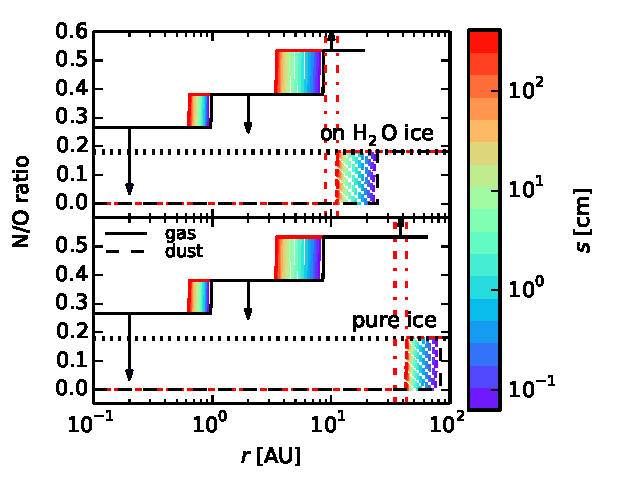
\includegraphics[width=0.5\textwidth]{N_O_water_ice.pdf}
%\vspace{-0.5in}
\caption{N/O ratio estimates in gas (solid lines) and dust (dashed lines) as function of semimajor axis in a viscous disk, for CO and N$_2$ residing in a water ice environment (top panel) or as pure ices (bottom panel). The H$_2$O, CO$_2$, CO and N$_2$ snowlines are shown for particles with initial sizes $\sim0.001$ cm $\lesssim s \lesssim$ 7 m as indicated by the color bar. The N/O ratio in a static disk (black lines) is shown for comparison. The arrows show that the N/O ratio in gas will decrease inside the H$_2$O and CO$_2$ snowlines in the viscous disk, as the relative fluxes of the desorbed icy
particles and the overall nebular gas will cause an excess of oxygen gas inside these snowlines (see Paper I for details). Radial drift and gas accretion move the N$_2$ snowline inward by up to $\sim$50\% compared to a static disk. The presence of N$_2$ in a water ice environment rather than as pure ice moves the N$_2$ snowline significantly inward by $\sim$70\%. The results of highly enhanced gas-phase N/O ratios in the outer disk compared to its average value, and of highly elevated N/O ratios in gas between the CO and N$_2$ snowlines (see Figure \ref{fig:Nstatic}), are preserved.}  
\label{fig:NO_ratio}
\end{figure}

%\emgr{Similar to the previous section, but with more details. Discuss that nitrogen is abundant in the solar system and disks and primarily found as N2. Due to the high volatility of N2, the gas phase N/O ratio in the outer disk may be even more enhanced than the C/O ratio. A fraction of the nitrogen abundance may be also carried by NH3. Discuss NH3 observed abundances and the choices that we make (no NH3, median, maximum). State that the NH3 desorption energy is only weakly dependent on whether it's pure NH3 or combined with H2O, but that is not the case for N2. Present new binding energies for N2 as pure ice and combined with water. Show Figure 4 and discuss how different nitrogen abundances and binding energies affect snowline locations and N/O ratio: N2 combined with H2O moves the N2 snowline inward by $\sim$50 AU (will calculate percentages too); the maximum reasonable abundance of NH3 changes the N/O ratio by $\sim$15\%. In the outer disk, the N/O ratio is enhanced by a factor of $\sim$4 compared to the solar value, twice as much as the C/O enhancement. Show Figure 5 and quantify the effect of drift and accretion on the NH3 snowline compared to a static disk. While NH3 does not have a significant effect on the N/O ratio in a static disk, this effect may be larger in a viscous disk, as the N gas abundance inside the NH3 snowline may be enhanced due to the differential motion of the desorbed ices and overall nebular gas (refer to Paper I). In this study, however, we neglect these effects and therefore do not include NH3 in estimating the N/O ratio (again, N/O ratio figure with drift is quite messy when including NH3 and does not add any information that is not already shown in Figures 4 and 5). Show Figure 6 and estimate the difference between N2-H2O and N2 pure ice snowlines in the case of drift, as well as the comparisons for the static disk for the N2 snowline. State that there will be an overabundance of gas-phase N/O between the CO and N2 snowlines, as there is no oxygen gas in this region.}



%\begin{figure}[h!]
%\centering
%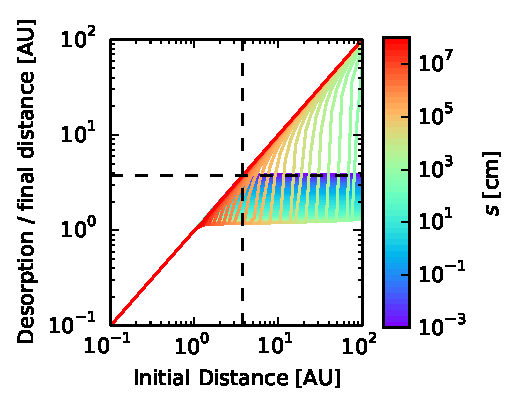
\includegraphics[width=0.5\textwidth]{../../figs/desorption_distance_NH3_steady.pdf}
%%\vspace{-0.5in}
%\caption{Desorption distance as a function of initial distance for NH3.... Drift and gas accretion move the NH3 snowline inward by x\%.} 
%\label{fig:NH3}
%\end{figure}

\subsection{N$_2$ Ice Environment and Disk Dynamics}

As in the case for CO, the N$_2$ binding energy is also strongly dependent on the ice environment in which the grain resides. If N$_2$ is a water dominated ice, the N$_2$ binding energy is 1266 K \citep{fayolle16}. Figure \ref{fig:NO_ratio} shows the H$_2$O, CO$_2$, CO and N$_2$ snowline locations in a viscous disk for particles with initial size $\sim0.06$ cm $\lesssim s \lesssim$ 7 m, and with the CO and N$_2$ snowlines calculated assuming different grain morphologies as explained above, as well as estimates for the N/O ratio throughout the disk. For simplicity, we assume that all nitrogen is bound in N$_2$. This choice is justified since the presence of some NH$_3$ only moderately changes the N/O ratio (see Figure \ref{fig:Nstatic}), and since we are primarily interested in the N$_2$ snowline locations rather than exact values for the N/O ratio. The innermost N$_2$ snowlines in the viscous disk, created by particles with $s \sim 7$ m for our fiducial model, are located at $r_{\rm N_2, pure} \approx 42$ AU for N$_2$ as pure ice and at $r_{\rm N_2, water} \approx 11$ AU for N$_2$ as water dominated ices. Compared to the static snowlines, i.e. $r_{\rm N_2, pure, static} \approx 79$ AU and $r_{\rm N_2, water, static} \approx 25$ AU, drift and gas accretion move the snowlines inward by up to $\sim$50 \%, similar to the case for CO (see Section \ref{sec:CH4}). By comparing our results in the viscous disk, we find that the N$_2$ snowline moves inward by more than 70\% if N$_2$ resides in a water ice environment rather than as pure ice. Similarly to the CO case, the N$_2$ snowline may move inward by a factor of $\sim$$7$ if we account for both disk dynamics and ice morphology (water dominated compared to pure), and may be close to or inward of 10 AU for certain disk models. 

\subsection{Implications for the Solar System}

%Our results for the N/O ratio imply that both gas phase and solid nitrogen abundances are enhanced in the outer disk, and that the regions in which these enhancements occur depend on disk dynamics and particle morphology. 

%The N$_2$ snowline moves inward by x\% in the pure ice scenario and by x\%.... 




%\section{Discussion}
%\label{sec:discussion}

%\emgr{Discuss how entrapment of volatiles by H2O affects volatile abundances and C/O ratios. Re-emphasize the fact that the C/O and N/O ratios are upper estimates, and that CH4 and NH3 might matter in a viscous disk. State that we plan to address this in a future paper. More TBD.}

\section{Summary}
\label{sec:summary}

In this paper we explore the role of icy grain morphology and disk dynamics on the snowline locations of major volatile carrier molecules and the C/N/O ratios in protoplanetary disks. We enhance the coupled drift-desorption model developed in \citet{piso15b} by adding more carbon- and nitrogen-bearing species into our framework and by considering different environments in which the icy grains reside. Our results can be summarized as follows:

\begin{enumerate}

\item Due to the high volatility of N$_2$, the gaseous N/O ratio in the outer disk is enhanced by more than a factor of three compared to its average value. This enhancement is more pronounced than in the case of the gas-phase C/O ratio, which is increased by a factor of two compared to the stellar value. Moreover, the N/O ratio in gas is expected to be very large between the CO and N$_2$ snowlines due to the complete depletion of oxygen gas in this region

\item The presence of some carbon in the form of CH$_4$ and of some nitrogen in the form of NH$_3$ only modestly affects our results for the C/O and N/O ratios, respectively. In both cases, large C/O and N/O ratios in the outer disk are preserved.

\item Grain composition sensitively affects the CO and N$_2$ snowline locations. If CO and N$_2$ are water dominated rather than pure ices, their snowlines move inward by up to $\sim$70 \%. This effect is separate from that of radial drift and viscous gas accretion, which also cause an inward movement of the CO and N$_2$ snowlines by up to $\sim$50 \%. 

\item The locations of the CO and N$_2$ snowlines are uncertain when we consider both viscous versus static disks, and pure versus water dominated ices. The snowlines in a viscous disk with CO or N$_2$ in a water environment are by up to a factor of $\sim$7 closer to the host star that in a static disk with CO or N$_2$ as pure ices. 

\end{enumerate}

Our results have direct consequences for the composition of nascent giant planets. The considerable inward movement of the CO and N$_2$ snowlines due to the ice grains residing in a water ice environment rather than as pure ices implies than giant planets with high C/O and/or N/O ratios in their atmospheres may form closer in than previously predicted by theoretical models. Moreover, our model shows that wide separation gas giants may have an excess of nitrogen in their envelopes, which may be used to trace their origins. In future work, we plan to add new levels of complexity to our model in terms of disk chemistry, dynamics, and planetary dynamics, thus forming a solid framework for understanding the origins of gas giants. 

%\emgr{Maybe we can include the summary in the discussion section?}

%\section{Volatile Abundances and Binding Energies: Effect on C/O and N/O Ratios in a Static Disk}
%
%\subsection{Nitrogen and CH4}
%
%\emgr{Discuss that nitrogen is abundant in the solar system and should be abundant in disks as well, but that its dominant form is largely unknown. Discuss that the main carrier of nitrogen is N2, but some fraction of it can be NH3 as well. Present and motivate the choices that we make for NH3 abundances. Along the same lines, discuss CH4, and the choices that we make for CH4 abundances.}
%
%\subsection{Volatile Desorption Energies}
%
%\emgr{State that desorption energies for H2O and CO2 are well constrained experimentally, and that the CO2 binding energy is only weakly dependent on whether it's pure CO2 or combined with H2O, but that is not the case for CO, N2 (and perhaps CH4 and NH3?). Briefly discuss CO-CO, N2-N2, CO-H2O and N2-H2O (and perhaps the same for CH4 and NH3 if we find literature on that) experimental results for binding energies, and motivate the choices that we make.}
%
%\subsection{Results for C/O and N/O in a Static Disk}
%
%\emgr{For each of them (C/O and N/O), show a 3-panel plot as follows: each panel has a specific CH4/NH3 abundance (top: none, middle: median abundance, bottom: maximum abundance); for a given panel, have multiple curves for C/O or N/O, depending on the choice of binding energies, so that it's clear visually how the binding energy changes the snowline location. Discuss how different abundances  and binding energies affect snowline locations and C/O or N/O ratios.}
%\section{Results}
%
%\subsection{N2, NH3 and CH4 Snowline Locations}
%
%\emgr{One multipanel 3x3 (or 3x2) rainbow plot similar to the snowline plots from Paper I, for \textit{one} choice for the binding energies (perhaps the largest ones, since we want a limit on how far in we can push the snowlines?). Rows: snowlines as a function or particle size for passive, active and (maybe) steady-state disk. Columns: N2, NH3 and CH4. Not entirely certain how necessary these plots/subsection actually are, since it is exactly the same qualitatively as in Paper I...}
%
%\subsection{C/O and N/O Ratios}
%
%\emgr{For each of them (C/O and N/O) show a 3x3 multipanel plot similar to the C/O plot from Paper I, for the same choice of binding energies as in the previous subsection. Columns: C/O or N/O in passive, active and steady-state disk. Rows: No CH4/NH3, median CH4/NH3, maximum CH4/NH3. Again, not sure if we need/want this for all disk choices, at least in the case of C/O since we already have that in Paper I. For N/O, quantify how the snowline location changes from a static disk due to drift and gas accretion.}






\if\bibinc n
\bibliography{refs}
\fi

\if\bibinc y
\begin{thebibliography}
\end{thebibliography}
\fi


\end{document}